\documentclass[10pt, xcolor=x11names]{beamer}
\usecolortheme{seagull}
\useoutertheme{infolines}
\usefonttheme[onlymath]{serif}
\setbeamertemplate{headline}[default]
\setbeamertemplate{navigation symbols}{}
\mode<beamer>{\setbeamertemplate{blocks}[rounded][shadow=true]}
\setbeamercovered{transparent}
\setbeamercolor{block body example}{fg=blue, bg=black!20}

\usepackage[utf8]{inputenc}
\usepackage[]{csquotes}
\usepackage{amsmath}
\usepackage{tikz, wasysym}
\usepackage{graphicx}
\usetikzlibrary{automata,positioning}
\usepackage{hyperref}
\usepackage{amsfonts}
\usepackage{csquotes}
\usepackage{tikz}
\usetikzlibrary{arrows}
\usetikzlibrary{arrows.meta}
\usepackage{wrapfig}
\usepackage{pgfplots}
\usepackage{outlines}
\usepackage{mathtools}
\usepackage{xcolor}



%\usepackage{amsfonts}
%\usepackage{amssymb}
%\usepackage{makeidx}
%\usepackage{graphicx}


\usepackage{hyperref}
\author{Sven Fiergolla}
\title[Colloquium]{Improving Run Length Encoding through preprocessing}
\subtitle[short version]{}
\date{14. Januar 2020}
%\institute[Uni Trier]{Universität Trier}
%\logo{\includegraphics[scale=.25]{unilogo.pdf}}

%read the data to \dataA
	


\begin{document}

	
	
	\frame{\maketitle}
	\frame{\frametitle{}
	\tableofcontents
	}



\section{Introduction}
\frame{\frametitle{Run Length Encoding (RLE)}
	\begin{outline}
		\1 employed in the transmission of analog television signals as far back as 1967
		\1 particularly well suited to palette-based bitmap images such as computer icons
	\end{outline}
}

\frame{\frametitle{Run Length Encoding (RLE)}
		assume $\Sigma = \{a,b\}$
	\[
	aaaaabbbbbbaaaaaabb
	\]
	\visible<2->{
		\[
		a^5b^6a^6b^2
		\]}
}

\frame{\frametitle{Run Length Encoding (RLE) - binary RLE}
	assume $\Sigma = \{a,b\}$
	\only<1-2>{
		\[
		aabaabbabbbababaabb
		\]
		\visible<2->{
			\[
			a^2b^1a^2b^2a^1b^3a^1b^1a^1b^1a^2b^2
			\]}}
	\only<3->{
		\only<3-9>{
		\[
		a^2b^1a^2b^2a^1b^3a^1b^1a^1b^1a^2b^2
		\]}
		\only<10>{\[
			\overbrace{a^2b^1a^2b^2a^1b^3a^1b^1a^1b^1a^2b^2}^{19 bit}
			\]}
		\visible<4->{
			\medskip \\
			assume $|\Sigma| = 2$ and runs start with $a$\\
			\visible<5->{
				set maximum run length to 3 ( $=2$ bits per run)\\
				\medskip
				\only<5>{
					\[
					212213111122
					\]}
				\only<6>{
					\[
					\underbrace{2}_{10}12213111122
					\]
				}
				\only<7>{
					\[
					\underbrace{2}_{10}\underbrace{1}_{01}2213111122
					\]
				}
				\only<8>{
					\[
					\underbrace{2}_{10}\underbrace{1}_{01}\underbrace{2}_{10}213111122
					\]
				}
				\only<9>{
					\[
					\underbrace{2}_{10}\underbrace{1}_{01}\underbrace{2}_{10}\underbrace{2}_{10}\underbrace{1}_{01}\underbrace{3}_{11}\underbrace{1}_{..}11122
					\]
}
				\only<10->{
	\[
	\overbrace{\underbrace{2}_{10}\underbrace{1}_{01}\underbrace{2}_{10}\underbrace{2}_{10}\underbrace{1}_{01}\underbrace{3}_{11}\underbrace{1}_{..}11122}^{24 bit}
	\]
}}}}}

\frame{\frametitle{Run Length Encoding (RLE) - binary RLE}
	assume $|\Sigma| = 2$ and runs start with $a$\\
	set maximum run length to 3 ( $=2$ bits per run / per RLE number)\\
	\visible<1>{
		\[
		b^1a^5b^2
		\]
	}
	\visible<2>{
		\[
		\underbrace{b^1}_{00 + 01}a^5b^2
		\]
	}
	\visible<3>{
		\[
		\underbrace{b^1}_{00 + 01} \: \: \underbrace{a^5}_{11 + 00 + 10}b^2
		\]
	}
	
	
}

\frame{\frametitle{Run Length Encoding (RLE) - byte wise RLE}
	assume $|\Sigma| > 2$\\
	set maximum run length to 4 ( $=2$ bits per run / per RLE number)\\
	\visible<1>{
		\[
		b^1a^2c^3
		\]
	}
	\visible<2>{
		\[
		\underbrace{b^1}_{01100010 + 00}a^2c^4
		\]
	}
	\visible<3>{
		\[
		\underbrace{b^1}_{01100010 + 00} \: \: \: \underbrace{a^2}_{01100001 + 01} \: \: \: \underbrace{c^3}_{01100011 + 11}
		\]
	}}

\frame{\frametitle{Run Length Encoding (RLE)}
	\begin{outline}
		\1 The International Telecommunication Union describes the standard to encode fax transmissions, known as T.45.
		\visible<2->{\2 RLE is combined with Huffman Encoding into \emph{Modified Huffman Encoding}.}
	\end{outline}
}


\frame{\frametitle{Huffman Encoding}
	\centering
	$w = cacbcacc$\\
	\visible<2->{$l_a(w) = 2 \:\:\: l_b(w) = 1 \:\:\: l_c(w) = 5$}
	\visible<3->{
	\begin{figure}[h]
		\centering
		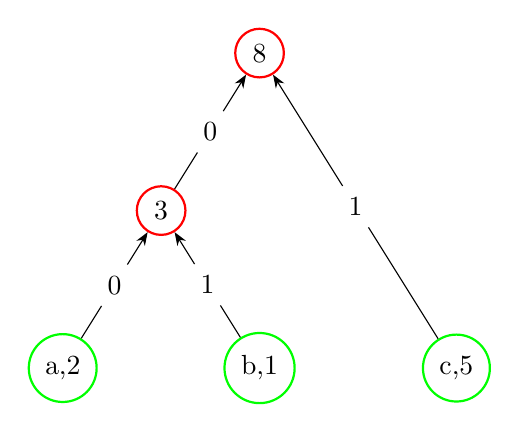
\begin{tikzpicture}
		\begin{scope}[every node/.style={circle,thick,draw=red}]
		\visible<4->{\node (B) at (1.25,2) {3};}
		\visible<5->{\node (C) at (2.5,4) {8};}
		\end{scope}
		\begin{scope}[every node/.style={circle,thick,draw=green}]
		\node (A) at (0,0) {a,2};
		\node (D) at (2.5,0) {b,1};
		\node (F) at (5,0) {c,5} ;
		\end{scope}
		
		\begin{scope}[>={Stealth[black]},
		every node/.style={fill=white,circle}]
		\visible<4->{\path [->] (A) edge node {$0$} (B);}
		\visible<5->{\path [->] (B) edge node {$0$} (C);}
		\visible<4->{\path [->] (D) edge node {$1$} (B);}
		\visible<5->{\path [->] (F) edge node {$1$} (C);}
		
		\end{scope}
		\end{tikzpicture}
		\caption{Example Huffman tree with 3 leaf nodes.} \label{fig:M1:example Huffman tree}
	\end{figure}
}
\visible<6->{$a = 00 \:\:\: b = 01 \:\:\: c = 1$}
}

\frame{\frametitle{Modified Huffman Encoding T.45}
	\begin{table}
		\centering
		\begin{tabular}[p]{r|c|c}
			run length &  white run Huffman codes & black run Huffman codes\\
			\hline
			0 &  00110101 & 0000110111\\
			1 & 000111 & 010\\
			2 & 0111 & 11\\
			3 & 1000 & 10\\
			4 & 1011 & 011\\
			... &  & \\
			20 & 0001000 & 00001101000\\
			... & & \\
			64+ & 11011 & 0000001111\\
			128+ & 10010 & 000011001000
			\label{tab:t1:static huffman codes}
		\end{tabular}
		\caption{T4 static Huffman codes.}
	\end{table}
	\only<2>{
		\[
		\underbrace{11111111111111111111}_{20} \rightarrow `00100`
		\]}
	\only<3->{
		\[
		0^{128} \rightarrow `10010` + `1011`
		\]}
}

\frame{\frametitle{Run Length Encoding (RLE)}
	\begin{outline}
		\1 The International Telecommunication Union describes the standard to encode fax transmissions, known as T.45.
		\2 RLE is combined with Huffman Encoding into \emph{Modified Huffman Encoding}.
		\1 RLE is also used for bitmap images or DNA sequence encoding.
	\end{outline}
}

\frame{\frametitle{Run Length Encoding (RLE)}
	\begin{table}[H]
		\centering
		\begin{tabular}{r|r|r|r|r|r}	
			file & size original & $\frac{bits}{\text{RLE number}}$ & size encoded & ratio in \% & \textit{bps}\\
			\hline
			pic & 513216 & 2 & 350292 & 68.25 & 5.46 \\
			& & 3 & 235067 & 45.80 & 3.66\\
			& & 4 & 165745 & 32.29 & 2.58\\
			& & 5 & 126349 & 24.61 & 1.96\\
			& & 6 & 106773 & 20.80 & 1.66\\
			& & 7 & 100098 & 19.50 & 1.56\\
			& & 8 & 101014 & 19.68 & 1.57\\		 
		\end{tabular}
		\caption{The file \textit{pic} with increasing bits per binary RLE encoded number.}
		\label{tab:t40 The file pic with increasing bits per RLE encoded number}
	\end{table}	
	\begin{itemize}
		\visible<2->{\item Byte-wise RLE achieves $27.2\%$ of its original size using 2.17 \textit{bps} with 6 bits per run.}
	\end{itemize}
}

\frame{\frametitle{Calgary Corpus}
	\begin{table}[H]
		\centering
		\begin{tabular}{l|r|l}	
			file & size & description\\
			\hline
			bib & 111261 & ASCII text - 725 bibliographic references\\
			book1 & 768771 & unformatted ASCII text\\
			book2 & 610856 & ASCII text in UNIX \enquote{troff} format\\
			geo & 102400 & 32 bit numbers in IBM floating point format\\
			news & 377109 & ASCII text - USENET batch file on a variety of topics\\
			obj1 & 21504 & VAX executable program \\
			obj2 & 246814 &	Macintosh executable program \\
			paper1 & 53161 & UNIX \enquote{troff} format \\
			paper2 & 82199 & UNIX \enquote{troff} format \\
			pic & 513216 & 1728 x 2376 bitmap image\\
			progc & 39611 & Source code in C \\
			progl & 71646 &  Source code in Lisp\\
			progp & 49379 & Source code in Pascal\\
			trans & 93695 & ASCII and control characters\\	 
		\end{tabular}
		\caption{The Calgary Corpus.}
		\label{tab:t05 The Calgary Corpus}
	\end{table}	
}


\frame{\frametitle{RLE - Unmodified compression on the Calgary Corpus}
	\begin{table}[h]
		\centering
		\begin{tabular}{l|r|r||r|r}
			bits per rle number & \multicolumn{2}{c}{byte-wise RLE} & \multicolumn{2}{c}{binary RLE} \\
			&  ratio in \% & \textit{bps} & ratio in \% & \textit{bps}\\
			\hline
			8 & 165 & 13.20 & 329 & 26.38\\
			7 & 154 & 12.38 & 288 & 23.11\\
			6 & 144 & 11.57 & 248 & 19.87 \\
			5 & 134 & 10.77 & 208 & 16.66\\
			4 & 125 & 10.00 & 168 & 13.51\\
			3 & 116 & 9.29 & 131 & 10.50\\
			2 & 109 & 8.74 & 104 & 8.36
		\end{tabular}
		\caption{Byte-wise and binary RLE on the Calgary Corpus.}
		\label{tab:t31 Byte-wise RLE on the Calgary Corpus}
	\end{table}
}

\frame{\frametitle{Findings}
	\begin{outline}
		\1 Files with long runs work really well with RLE.
		\visible<2->{\1 Most files other than pallet based images do not contain long runs of identical bit values.}
		\medskip
		\visible<3->{\1 Artificially creating runs on arbitrary data will improve the performance of RLE.}
	\end{outline}	
}

\section{Basics}
\frame{\frametitle{Basics of Compression}
	\begin{itemize}
		\item Non random data contains redundant information
		\item Compression is about pattern or structure identification and exploitation
		
		\visible<2->{  \item No algorithm can compress all possible data of a given length, even by one byte (Kolmogorov Complexity)}
	\end{itemize}	
}

\frame{\frametitle{Basics of Compression - Entropy Encoding}
	\begin{itemize}
		\item generating a probability model for the data
		\item compute variable length codes	
		\visible<2->{ \item low speed, high compression strength
		\item recommended for poorly structured data}
	\end{itemize}	
}

\frame{\frametitle{Basics of Compression - Entropy Encoding}
\begin{outline}
		\1 Huffman Encoding (1952)
		\2 computes optimal length prefix-free codes for symbols acc. to their probabilities
		\visible<2->{ \1 Run Length Encoding (1967) \2 computes runs of identical symbols}
		\visible<3->{ \1 Arithmetic Encoding (1979) \2 encodes a message of symbols in a single rational number in [0,1]}
		\visible<4->{\1 Asymmetric Numeral Systems (ANS) Encoding (2014) \2 encodes a message of symbols in a single natural number}
\end{outline}
}

\frame{\frametitle{Basics of Compression - Dictionary Encoding}
	\begin{outline}
		\1 maintain a dictionary of strings for either a \emph{sliding window} or the whole data
		\2 replace later occurrence with reference position an length
		\visible<2->{ \1 High speed, moderate compression strength}
		\visible<3->{ \1 Famous Lempel-Ziv methods LZ77 and LZ78 (1977/78) \2 many derivatives, some still used today}
	\end{outline}
}

\frame{\frametitle{State of the art}
	\begin{table}[h]
	\begin{tabular}{r|r|r|r|r}
		method & options &  size in bytes & compression & \textit{bps}\\
		\hline
		uncompressed & & 3,145,718 & 100.0\% & 8.00 \\
		compress 4.2.4 & & 1,250,382 & 40.4\% & 3.24 \\
		gzip v1.10 & -9 & 1,021,720 & 32.4\% & 2.60\\
		ZIP v3.0 &-9& 1,019,783 & 32.4\% & 2.59 \\
		zstandard 1.4.2& --ultra-23 -long=30 & 887,004 & 28.1\% & 2.25\\
		bzip2 v1.0.8 & --best & 832,443 & 26.4\% & 2.11 \\
		brotli 1.0.7 & -q 11 -w 24 & 826,638 & 26.3\%& 2.10\\
		p7zip 16.02 (deflate) & a -mx10 & 821,873 & 26.1\% & 2.08 \\
		p7zip 16.02 (PPMd) & a -mm=ppmd o=32 & 763,067& 24.2\% & 1.93 \\
		ZPAQ v7.15 & -m5 & 659,700 & 20.9\% & 1.67  \\
		paq8hp* & - & - & - & - \\
		cmix v18 & -c -d & 554,983 & 17.6\% & 1.41 		
	\end{tabular}
	\label{tab:t20 stat of the art}
	\caption{State of the art compression ratios on the Calgary Corpus.}
\end{table}
}


\section{Design}
\frame{\frametitle{Design - Preprocessing}
	\begin{outline}
		\1 Vertical interpretation of the input
		\visible<2->{\1 Dynamic byte remapping}
		\visible<3->{\1 Burrows-Wheeler-Transformation}
		\visible<4->{\1 Huffman Encoding of runs}
	\end{outline}	
}

\frame{\frametitle{Preprocessing - Vertical interpretation}
	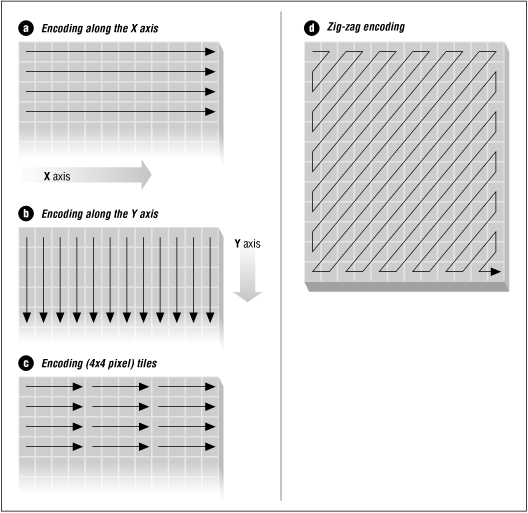
\includegraphics[height=\textheight, width=\textwidth]{g0902.png}
}

	\frame{\frametitle{Preprocessing - Vertical interpretation}
		\[
			S = abraca
		\]
		\only<1>{
		\textcolor{red}{0} 1 1 0 0 0 0 1 
		0 1 1 0 0 0 1 0 
		0 1 1 1 0 0 1 0 
		0 1 1 0 0 0 0 1 
		0 1 1 0 0 0 1 1 
		0 1 1 0 0 0 0 1 
	}
		\only<2>{
	0 \textcolor{red}{1} 1 0 0 0 0 1 
	0 1 1 0 0 0 1 0 
	0 1 1 1 0 0 1 0 
	0 1 1 0 0 0 0 1 
	0 1 1 0 0 0 1 1 
	0 1 1 0 0 0 0 1 
}
		\only<3>{
	0 1 \textcolor{red}{1} 0 0 0 0 1 
	0 1 1 0 0 0 1 0 
	0 1 1 1 0 0 1 0 
	0 1 1 0 0 0 0 1 
	0 1 1 0 0 0 1 1 
	0 1 1 0 0 0 0 1 
}
		\only<4>{
	0 1 1 \textcolor{red}{0} 0 0 0 1 
	0 1 1 0 0 0 1 0 
	0 1 1 1 0 0 1 0 
	0 1 1 0 0 0 0 1 
	0 1 1 0 0 0 1 1 
	0 1 1 0 0 0 0 1 
}

}
	
\frame{\frametitle{Preprocessing - Vertical interpretation}
	\only<1>{
\begin{equation}
\begin{multlined}
	S = abraca\\
		\textcolor{red}{0} 1 1 0 0 0 0 1 \\
		0 1 1 0 0 0 1 0 \\
		0 1 1 1 0 0 1 0 \\
		0 1 1 0 0 0 0 1 \\
		0 1 1 0 0 0 1 1 \\
		0 1 1 0 0 0 0 1 \\
\end{multlined}
\end{equation}
}
	\only<2>{
	\begin{equation}
	\begin{multlined}
	S = abraca\\
	0 1 1 0 0 0 0 1 \\
	\textcolor{red}{0} 1 1 0 0 0 1 0 \\
	0 1 1 1 0 0 1 0 \\
	0 1 1 0 0 0 0 1 \\
	0 1 1 0 0 0 1 1 \\
	0 1 1 0 0 0 0 1 \\
	\end{multlined}
	\end{equation}
}

	\only<3>{
	\begin{equation}
	\begin{multlined}
	S = abraca\\
	0 1 1 0 0 0 0 1 \\
	0 1 1 0 0 0 1 0 \\
	\textcolor{red}{0} 1 1 1 0 0 1 0 \\
	0 1 1 0 0 0 0 1 \\
	0 1 1 0 0 0 1 1 \\
	0 1 1 0 0 0 0 1 \\
	\end{multlined}
	\end{equation}
}

	\only<4>{
	\begin{equation}
	\begin{multlined}
	S = abraca\\
	0 1 1 0 0 0 0 1 \\
	0 1 1 0 0 0 1 0 \\
	0 1 1 1 0 0 1 0 \\
	\textcolor{red}{0} 1 1 0 0 0 0 1 \\
	0 1 1 0 0 0 1 1 \\
	0 1 1 0 0 0 0 1 \\
	\end{multlined}
	\end{equation}
}
	\only<5>{
	\begin{equation}
	\begin{multlined}
	S = abraca\\
	0 1 1 0 0 0 0 1 \\
	0 1 1 0 0 0 1 0 \\
	0 1 1 1 0 0 1 0 \\
	0 1 1 0 0 0 0 1 \\
	\textcolor{red}{0} 1 1 0 0 0 1 1 \\
	0 1 1 0 0 0 0 1 \\
	\end{multlined}
	\end{equation}
}

	\only<6>{
	\begin{equation}
	\begin{multlined}
	S = abraca\\
	0 1 1 0 0 0 0 1 \\
	0 1 1 0 0 0 1 0 \\
	0 1 1 1 0 0 1 0 \\
	0 1 1 0 0 0 0 1 \\
	0 1 1 0 0 0 1 1 \\
	\textcolor{red}{0} 1 1 0 0 0 0 1 \\
	\end{multlined}
	\end{equation}
}
	\only<7>{
	\begin{equation}
	\begin{multlined}
	S = abraca\\
	0 \textcolor{red}{1} 1 0 0 0 0 1 \\
	0 1 1 0 0 0 1 0 \\
	0 1 1 1 0 0 1 0 \\
	0 1 1 0 0 0 0 1 \\
	0 1 1 0 0 0 1 1 \\
	0 1 1 0 0 0 0 1 \\
	\end{multlined}
	\end{equation}
}

	\only<8>{
	\begin{equation}
	\begin{multlined}
	S = abraca\\
	0 1 1 0 0 0 0 1 \\
	0 \textcolor{red}{1} 1 0 0 0 1 0 \\
	0 1 1 1 0 0 1 0 \\
	0 1 1 0 0 0 0 1 \\
	0 1 1 0 0 0 1 1 \\
	0 1 1 0 0 0 0 1 \\
	\end{multlined}
	\end{equation}
}}

\frame{\frametitle{Preprocessing - Vertical interpretation}
	\begin{table}[H]
		\centering
		\begin{tabular}{r|r|r}	
			bits per rle number & ratio in \% & \textit{bps}\\
			\hline
			8 & 255.22 & 20.41\\
			7 & 224.45 & 17.95\\
			6 & 194.74 & 15.57\\
			5 & 167.04 & 13.36\\
			4 & 142.58 & 11.40\\
			3 & 127.80 & 10.22\\
			2 & 139.79 & 11.18 \\
		\end{tabular}
		\caption{Binary RLE on vertical interpreted data, fixed run lengths.}
		\label{tab:t30 binary RLE on vertical interpreted data}
	\end{table}
}

\frame{\frametitle{Preprocessing - Vertical interpretation}
	\centering
	8 bits per run
	\begin{math}
	\left\{
	\left.
	\begin{array}{l}
0 1 1 0 0 0 0 1 \\
0 1 1 0 0 0 1 0 \\
0 1 1 1 0 0 1 0 \\
0 1 1 0 0 0 0 1 \\
0 1 1 0 0 0 1 1 \\
0 1 1 0 0 0 0 1\\
	\end{array}
	\right \}
	\right.
	\end{math}
	2 bits per run
}

\frame{\frametitle{Preprocessing - Vertical interpretation}
\begin{figure}[h]
	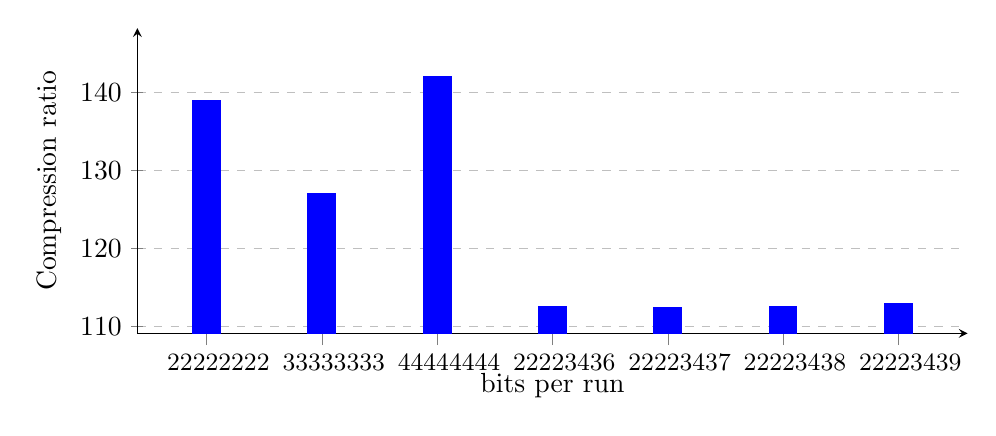
\begin{tikzpicture}
	\begin{axis}[
	width=\textwidth,
	height=0.45\textwidth,
	axis x line=center,
	axis y line=left,
	xlabel={bits per run},
	ylabel={Compression ratio},
	symbolic x coords = {22222222,33333333,44444444,22223436,22223437,22223438,22223439,22233578,22233579,222335710},
	x tick label style={font=\small,text width=1cm,align=center},
	xtick=data,
	x label style={at={(axis description cs:0.5,-0.1)},anchor=north},
	enlargelimits=true,
	ymax=145,
	legend style={
		at={(0.5,1.2)},
		anchor=north,
		legend columns=-1,
		/tikz/every even column/.append style={column sep=0.5cm}
	},	
	ymajorgrids=true,
	grid style=dashed,
	ybar]
	\addplot[color=blue,fill]
	coordinates {
		(22222222,139)(33333333,127)(44444444,142)(22223436,112.55)(22223437,112.4)(22223438,112.6)(22223439,113)
	};
	\end{axis}
	\end{tikzpicture}
	%}
	%\end{scaletikzpicturetowidth}
	\caption{Byte mapping and varying maximum run lengths.}
	\label{fig:2:Byte mapping and varying maximum run lengths}
\end{figure}
}

\frame{\frametitle{Preprocessing - Vertical interpretation}
\begin{table}[h]
	\centering
	\begin{tabular}{r|r|r|r|r}	
		file & size original & size encoded & ratio in \% & \textit{bps}\\
		\hline
		bib & 111261 & 129424 & 116.32 & 9.31 \\
		book1 & 768771 & 820463 & 106.72 & 8.54 \\
		book2 & 610856 & 659811 & 108.01 & 8.64 \\
		geo & 102400 & 162274 & 158.47 & 12.68 \\
		news & 377109 & 400810 & 106.28 & 8.50 \\
		obj1 & 21504 & 31592 & 146.91 & 11.75 \\
		obj2 & 246814 & 379591 & 153.80 & 12.30 \\
		paper1 & 53161 & 57654 & 108.45 & 8.68 \\
		paper2 & 82199 & 88121 & 107.20 & 8.58 \\
		pic & 513216 & 533254 & 103.90 & 8.31 \\
		progc & 39611 & 41360 & 104.42 & 8.35 \\
		progl & 71646 & 74554 & 104.06 & 8.32 \\
		progp & 49379 & 53403 & 108.15 & 8.65 \\
		trans & 93695 & 99818 & 106.54 & 8.52 \\
		\hline
		all files & 3145718 & 3536225 & 112.41 & 8.99
	\end{tabular}
	\caption{Calgary Corpus encoded, vertical encoding, using bits per run (2, 2, 2, 2, 3, 4, 3, 7).}
	\label{tab:t50:Calgary Corpus encoded, vertical encoding, using bits per run: (2, 2, 2, 2, 3, 4, 3, 7)}
\end{table}
}


\frame{\frametitle{Preprocessing - Byte Remapping}
	\begin{equation}
	\begin{multlined}
	S = abraca\\
	0 1 1 0 0 0 0 1 \\
	0 1 1 0 0 0 1 0 \\
	0 1 1 1 0 0 1 0 \\
	0 1 1 0 0 0 0 1 \\
	0 1 1 0 0 0 1 1 \\
	0 1 1 0 0 0 0 1 \\
	\end{multlined}
	\end{equation}
}

\frame{\frametitle{Preprocessing - Byte Remapping}
	\begin{equation}
	\begin{multlined}
	S = abraca\\
	0 0 0 0 0 0 0 0 \\
	0 0 0 0 0 0 0 1 \\
	0 0 0 0 0 0 1 1 \\
	0 0 0 0 0 0 0 0 \\
	0 0 0 0 0 0 1 0 \\
	0 0 0 0 0 0 0 0 \\
	\end{multlined}
	\end{equation}
}



\frame{\frametitle{Preprocessing - Byte Remapping}
	\begin{figure}[h]
		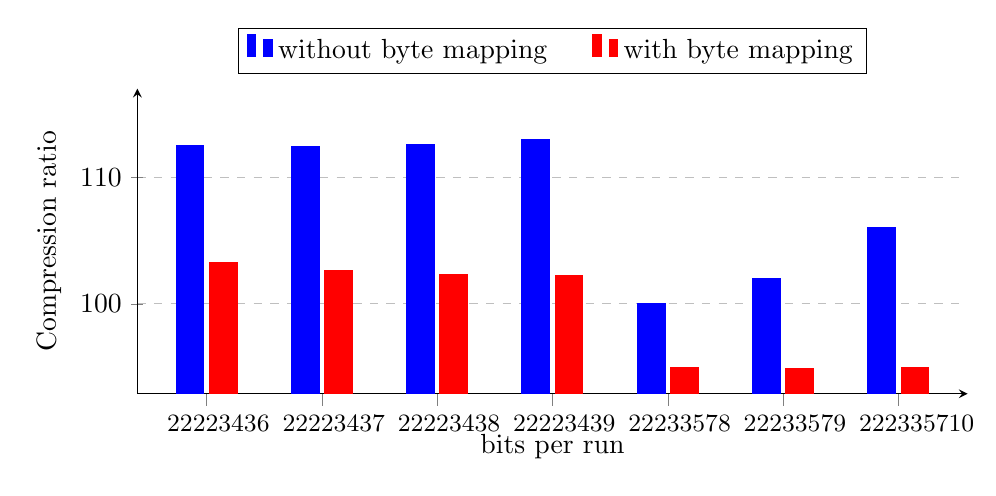
\begin{tikzpicture}
		\begin{axis}[
		width=\textwidth,
		height=0.45\textwidth,
		axis x line=center,
		axis y line=left,
		xlabel={bits per run},
		ylabel={Compression ratio},
		symbolic x coords={22223436,22223437,22223438,22223439,22233578,22233579,222335710},
		x tick label style={font=\small,text width=1cm,align=center},
		xtick=data,
		x label style={at={(axis description cs:0.5,-0.1)},anchor=north},
		enlargelimits=true,
		ymax=115,
		legend style={
			at={(0.5,1.2)},
			anchor=north,
			legend columns=-1,
			/tikz/every even column/.append style={column sep=0.5cm}
		},	
		ymajorgrids=true,
		grid style=dashed,
		ybar]
		\addplot[color=blue,fill]
		coordinates {
			(22223436,112.55)(22223437,112.4)(22223438,112.6)(22223439,113)(22233578,100)(22233579,102)(222335710,106)
		};
		\addplot[color=red,fill]
		coordinates {
			(22223436,103.3)(22223437,102.6)(22223438,102.3)(22223439,102.25)(22233578,95)(22233579,94.9)(222335710,95)
		};
		\legend{without byte mapping,with byte mapping}
		\end{axis}
		\end{tikzpicture}
		%}
		%\end{scaletikzpicturetowidth}
		\caption{Byte mapping and varying maximum run lengths.}
		\label{fig:2:Byte mapping and varying maximum run lengths2}
	\end{figure}
}

\frame{\frametitle{Preprocessing - Byte Remapping}
\begin{table}[h]
	\centering
	\begin{tabular}{r|r|r|r|r}	
		file & size original & size encoded & ratio in \% & \textit{bps}\\
		\hline
		bib & 111261 & 111579 & 100.29 & 8.02 \\
		book1 & 768771 & 669578 & 87.10 & 6.97 \\
		book2 & 610856 & 551757 & 90.33 & 7.23 \\
		geo & 102400 & 144974 & 141.58 & 11.33 \\
		news & 377109 & 363010 & 96.26 & 7.70 \\
		obj1 & 21504 & 30166 & 140.28 & 11.22 \\
		obj2 & 246814 & 340165 & 137.82 & 11.03 \\
		paper1 & 53161 & 50074 & 94.19 & 7.54 \\
		paper2 & 82199 & 71747 & 87.28 & 6.98 \\
		pic & 513216 & 408136 & 79.53 & 6.36 \\
		progc & 39611 & 38490 & 97.17 & 7.77 \\
		progl & 71646 & 63765 & 89.00 & 7.12 \\
		progp & 49379 & 46093 & 93.35 & 7.47 \\
		trans & 93695 & 94729 & 101.10 & 8.09 \\
		\hline
		all files & 3145718 & 2988359 & 94.99 & 7.59
	\end{tabular}
	\caption{Calgary Corpus encoded with vertical reading, byte remapping, using bits per run (2, 2, 3, 3, 3, 4, 5, 8).}
	\label{tab:t43 Calgary Corpus encoded with vertical reading, byte remapping and varying bits per run}
\end{table}	
}
\frame{\frametitle{Preprocessing - Burrows-Wheeler-Transformation}
TODO	
}
\frame{\frametitle{Preprocessing - Burrows-Wheeler-Transformation}
	
	\[
		S = abcabr
	\]
	
		\only<1>{
			\begin{table}[h]
				\centering
				\begin{tabular}{r|l|l|l|l|l|l}
					row 1 & a & b & c & a & b & r\\
					\hline
					row 2 & r & a & b & c & a & b\\	
					\hline
					row 3 & b & r & a & b & c & a\\
					\hline
					row 4 & a & b & r & a & b & c\\
					\hline
					row 5 & c & a & b & r & a & b\\
					\hline
					row 6 & b & c & a & b & r & a
						\label{tab:t10 bwt-example1}
				\end{tabular}
				\caption{Burrows Wheeler Transformation Matrix (all cyclic rotations).}
			\end{table}
		}
	\only<2>{
	\begin{table}[h]
		\centering
		\begin{tabular}{r|l|l|l|l|l|l}
			row 1 & a & b & c & a & b & r\\
			\hline
			row 2 & a & b & r & a & b & c\\
			\hline
			row 3 & b & c & a & b & r & a\\
			\hline
			row 4 & b & r & a & b & c & a\\
			\hline
			row 5 & c & a & b & r & a & b\\
			\hline
			row 6 & r & a & b & c & a & b	
			\label{tab:t10 bwt-example2}
		\end{tabular}
		\caption{Burrows Wheeler Transformation Matrix (all cyclic rotations, sorted).}
	\end{table}
}
	\only<3>{
		\begin{table}[h]
			\centering
			\begin{tabular}{r|l|l|l|l|l|l}
				row 1 & a & b & c & a & b & \textcolor{red}{r}\\
				\hline
				row 2 & a & b & r & a & b &  \textcolor{red}{c}\\
				\hline
				row 3 & b & c & a & b & r &  \textcolor{red}{a}\\
				\hline
				row 4 & b & r & a & b & c &  \textcolor{red}{a}\\
				\hline
				row 5 & c & a & b & r & a &  \textcolor{red}{b}\\
				\hline
				row 6 & r & a & b & c & a &  \textcolor{red}{b}
				\label{tab:t10 bwt-example3}
			\end{tabular}
			\caption{Burrows Wheeler Transformation Matrix (all cyclic rotations, sorted).}
		\end{table}
		 \[
		 L = rcaabb
		 \]
		 \[
		 i = 1
		 \]
	}
}

\frame{\frametitle{Preprocessing - inverse Burrows-Wheeler-Transformation}
		 \[
		 L = rcaabb
		 \]
		 \[
		 i = 1
		 \]
		 \visible<2->{
		 \begin{table}[h]
		 	\centering
		 	\begin{tabular}{l|l|l}
		 		word & word with position & sorted\\
		 		\hline
		 		r & (r,1) & (a,3) \\
		 		c & (c,2) & (a,4) \\
		 		a & (a,3) & (b,5) \\
		 		a & (a,4) & (b,6) \\
		 		b & (b,5) & (c,2) \\
		 		b & (b,6) & (r,1)
		 		\label{tab:t11 standard permutation}
		 	\end{tabular}
		 	\caption{Standard permutation generation of the word $L$.}
		 \end{table}
		}
}

\frame{\frametitle{Preprocessing - inverse Burrows-Wheeler-Transformation}
		 \[
		 L = rcaabb
		 \]
		 \[
		 i = 1
		 \]
	This yields a standard permutation of:
	\begin{gather}  
	\pi_L = 
	\begin{pmatrix} 1 & 2 & 3 & 4 & 5 & 6\\ 3 & 4 & 5 & 6 & 2 & 1 \end{pmatrix}
	\end{gather}
	\visible<2->{
	Following $\pi^1_L(1)$ to $\pi^6_L(1)$ :
	\begin{gather} 
	3 \xrightarrow[]{\pi_L} 5 \xrightarrow[]{\pi_L} 2 \xrightarrow[]{\pi_L} 4 \xrightarrow[]{\pi_L} 6 \xrightarrow[]{\pi_L} 1 
	\end{gather}}

	\visible<3->{
	Applying the sequence to the labeling function of the word $L$:
	\begin{gather}  
	\lambda_L(3) \: \lambda_L(5) \: \lambda_L(2) \: \lambda_L(4) \: \lambda_L(6) \: \lambda_L(1)
	= abcabr = w
	\end{gather}}
}

\frame{\frametitle{Preprocessing - Burrows-Wheeler-Transformation}
\begin{table}[h]
	\centering
	\begin{tabular}{r|r|r}	
		bits per rle number & ratio in \% & \textit{bps}\\
		\hline
		3 & 95.41 & 7.63\\
		2 & 91.39 & 7.31 \\
	\end{tabular}
	\caption{Initial BWT implementation on byte wise RLE.}
	\label{tab:t11 Simple Burrows Wheeler Transformation on byte wise RLE}
\end{table}	

\visible<2->{
\begin{table}[h]
	\centering
	\begin{tabular}{r|r|r}	
		bits per rle number & ratio in \% & \textit{bps}\\
		\hline
		3 & 91.62 & 7.33\\
		2 & 89.46 & 7.15
	\end{tabular}
	\caption{Burrows Wheeler Transformation on byte wise RLE.}
	\label{tab:t12 Burrows Wheeler Transformation on byte wise RLE}
\end{table}}
}

\frame{\frametitle{Preprocessing - Burrows-Wheeler-Transformation}
	\begin{table}[h]
		\centering
		\begin{tabular}{r|r|r}	
			bits per rle number & ratio in \% & \textit{bps}\\
			\hline
			8 & 74.42 & 5.95\\
			7 & 69.90 & 5.59\\
			6 & 65.58 & 5.24\\
			5 & 61.71 & 4.93\\
			4 & 58.98 & 4.71\\
			3 & 59.18 & 4.73\\
			2 & 67.69 & 5.41
		\end{tabular}
		\caption{Modified Burrows Wheeler Transformation on byte wise RLE.}
		\label{tab:t13 Modified Burrows Wheeler Transformation on byte wise RLE}
	\end{table}	
}

\frame{\frametitle{Preprocessing - Burrows-Wheeler-Transformation}
\begin{table}[h]
	\centering
	\begin{tabular}{r|r|r|r|r}	
		file & size original & size encoded & compression & \textit{bps}\\
		\hline
		bib & 111261 & 59285 & 53.28 & 4.26 \\
		book1 & 768771 & 590879 & 76.86 & 6.15 \\
		book2 & 610856 & 374742 & 61.35 & 4.91 \\
		geo & 102400 & 101192 & 98.82 & 7.91 \\
		news & 377109 & 246047 & 65.25 & 5.22 \\
		obj1 & 21504 & 16467 & 76.58 & 6.13 \\
		obj2 & 246814 & 126626 & 51.30 & 4.10 \\
		paper1 & 53161 & 34130 & 64.20 & 5.14 \\
		paper2 & 82199 & 56507 & 68.74 & 5.50 \\
		pic & 513216 & 136074 & 26.51 & 2.12 \\
		progc & 39611 & 24312 & 61.38 & 4.91 \\
		progl & 71646 & 31466 & 43.92 & 3.51 \\
		progp & 49379 & 20862 & 42.25 & 3.38 \\
		trans & 93695 & 32835 & 35.04 & 2.80 \\
		\hline
		all files & 3145718 & 1855520 & 58.98 & 4.71
	\end{tabular}
	\caption{Calgary Corpus encoded with byte wise RLE after a Burrows-Wheeler- Transformation with 4 bit per run.}
	\label{tab:t14:Calgary Corpus encoded with byte wise RLE after a Burrows-Wheeler-Transformation}
\end{table}	
}

\frame{\frametitle{Preprocessing - Burrows-Wheeler-Transformation}
\begin{figure}[h]
	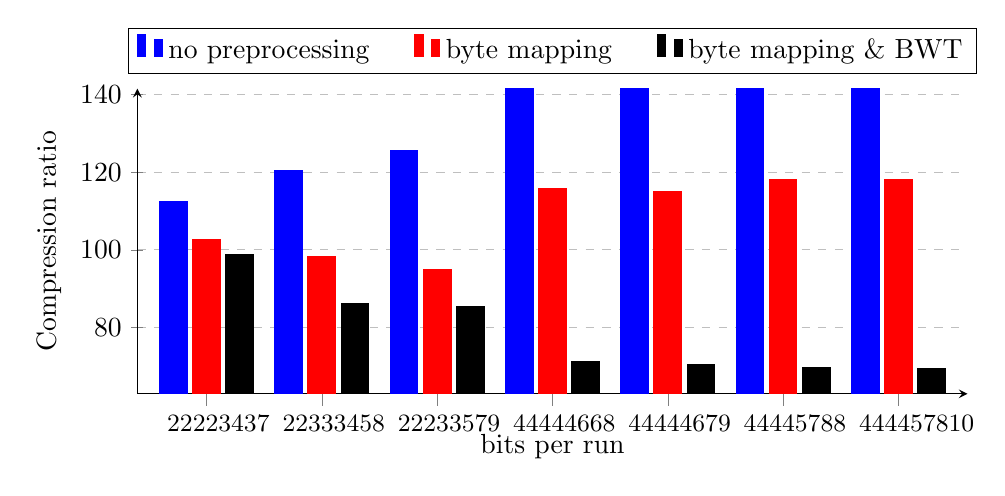
\begin{tikzpicture}
	\begin{axis}[
	width=\textwidth,
	height=0.45\textwidth,
	axis x line=center,
	axis y line=left,
	xlabel={bits per run},
	x label style={at={(axis description cs:0.5,-0.1)},anchor=north},
	ylabel={Compression ratio},
	symbolic x coords={22223437,22333458,22233579,44444668,44444679,44445788,444457810},
	x tick label style={font=\small,text width=1cm,align=center},
	xtick=data,
	enlargelimits=true,
	ymax=135,
	legend style={
		at={(0.5,1.2)},
		anchor=north,
		legend columns=-1,
		/tikz/every even column/.append style={column sep=0.5cm}
	},	
	ymajorgrids=true,
	grid style=dashed,
	ybar
	]
	\addplot[color=blue,fill]
	coordinates {
		(22223437,112.4)(22333458,120.4 )(22233579,125.6)(44444668,147.2)(44444679,151.3)(44445788,159.7)(444457810,160.8)
	};
	\addplot[color=red,fill]
	coordinates {
		(22223437,102.6)(22333458,98.2 )(22233579,94.99)(44444668,115.7)(44444679,115.1)(44445788,118)(444457810,118)
	};
	\addplot[color=black,fill]
	coordinates {
		(22223437,98.8)(22333458,86.1 )(22233579,85.3)(44444668,71.2)(44444679,70.3)(44445788,69.6)(444457810,69.4)
	};
	\legend{no preprocessing,byte mapping,byte mapping \& BWT}
	\end{axis}
	\end{tikzpicture}
	%}
	%\end{scaletikzpicturetowidth}
	\caption{Byte mapping and varying maximum run lengths, all preprocessing steps.}
	\label{fig:3:Different run lengths with and without transformations}
\end{figure}
}


\frame{\frametitle{Preprocessing - Burrows-Wheeler-Transformation}
\begin{table}[h]
	\centering
	\begin{tabular}{r|r|r|r|r}	
		file & size original & size encoded & ratio in \% & \textit{bps}\\
		\hline
		bib & 111261 & 73843 & 66.37 & 5.31 \\
		book1 & 768771 & 570348 & 74.19 & 5.94 \\
		book2 & 610856 & 409639 & 67.06 & 5.36 \\
		geo & 102400 & 145950 & 142.53 & 11.40 \\
		news & 377109 & 275396 & 73.03 & 5.84 \\
		obj1 & 21504 & 27023 & 125.66 & 10.05 \\
		obj2 & 246814 & 213392 & 86.46 & 6.92 \\
		paper1 & 53161 & 37344 & 70.25 & 5.62 \\
		paper2 & 82199 & 56490 & 68.72 & 5.50 \\
		pic & 513216 & 227914 & 44.41 & 3.55 \\
		progc & 39611 & 28275 & 71.38 & 5.71 \\
		progl & 71646 & 38144 & 53.24 & 4.26 \\
		progp & 49379 & 27029 & 54.74 & 4.38 \\
		trans & 93695 & 49314 & 52.63 & 4.21 \\
		\hline
		all files & 3145718 & 2184197 & 69.43 & 5.55
	\end{tabular}
	\caption{Calgary Corpus encoded, byte mapping and a BWTS as preprocessing, using bits per run (4, 4, 4, 4, 5, 7, 8, 10).}
	\label{tab:t5:Calgary Corpus encoded, all preprocessing steps, using bits per run: 4, 4,4, 4, 5, 7, 8, 10}
\end{table}
}

\frame{\frametitle{Preprocessing - Huffman Encoding RLE runs}
	
}

\frame{\frametitle{Preprocessing - Huffman Encoding RLE runs}
		\begin{table}[H]
			\centering
			\begin{tabular}{r|r|r|r|r}	
				file & size original & size encoded & ratio in \% & \textit{bps}\\
				\hline
				bib & 111261 & 44156 & 39.69 & 3.17 \\
				book1 & 768771 & 340279 & 44.26 & 3.54 \\
				book2 & 610856 & 243092 & 39.80 & 3.18 \\
				geo & 102400 & 63006 & 61.53 & 4.92 \\
				news & 377109 & 173207 & 45.93 & 3.67 \\
				obj1 & 21504 & 14405 & 66.99 & 5.36 \\
				obj2 & 246814 & 119957 & 48.60 & 3.89 \\
				paper1 & 53161 & 24917 & 46.87 & 3.75 \\
				paper2 & 82199 & 35939 & 43.72 & 3.50 \\
				pic & 513216 & 82136 & 16.00 & 1.28 \\
				progc & 39611 & 18890 & 47.69 & 3.82 \\
				progl & 71646 & 24649 & 34.40 & 2.75 \\
				progp & 49379 & 17416 & 35.27 & 2.82 \\
				trans & 93695 & 31235 & 33.34 & 2.67 \\
				\hline
				all files & 3145718 & 1237380 & 39.33 & 3.14
			\end{tabular}
			\caption{Calgary Corpus encoded with vertical reading, byte mapping and a BWTS as preprocessing, using Huffman encoding for all counted runs, 8 bit per run.}
			\label{tab:t6:Calgary Corpus encoded, all preprocessing steps, using Huffman encoding for all counted runs}
		\end{table}
}

\section{Implementation}
\frame{\frametitle{Implementation}
TODO	
}
\section{Evaluation and Discussion}
\frame{\frametitle{Evaluation and Discussion}
TODO	
}
\frame{\frametitle{Evaluation and Discussion}
		\begin{table}[h]
			\centering
			\begin{tabular}{r|r|r|r|r}	
				file & size original & size encoded & ratio in \% & \textit{bps}\\
				\hline
				alice29.txt & 152089 & 65445 & 43.03 & 3.44 \\
				asyoulik.txt & 125179 & 59291 & 47.36 & 3.79 \\
				cp.html & 24603 & 11073 & 45.01 & 3.60 \\
				fields.c & 11150 & 5183 & 46.48 & 3.72 \\
				grammar.lsp & 3721 & 1923 & 51.68 & 4.13 \\
				kennedy.xls & 1029744 & 229823 & 22.32 & 1.79 \\
				lcet10.txt & 426754 & 170593 & 39.97 & 3.20 \\
				plrabn12.txt & 481861 & 215628 & 44.75 & 3.58 \\
				ptt5 & 513216 & 82136 & 16.01 & 1.28 \\
				sum & 38240 & 19616 & 51.30 & 4.10 \\
				xargs.1 & 4227 & 2515 & 59.50 & 4.76 \\
				\hline
				all files & 2814880 & 867322 & 30.81 & 2.46
			\end{tabular}
			\caption{Canterbury encoded, all preprocessing steps, using Huffman encoding for all counted runs.}
			\label{tab:t100:Canterbury encoded, all preprocessing steps, using Huffman encoding for all counted runs}
		\end{table}
}
\frame{\frametitle{Evaluation and Discussion}
		\begin{table}[h]
			\begin{tabular}{r|r|r|r|r|r}
				method  &  size in bytes & compression & \textit{bps} & \multicolumn{2}{c}{time }\\
				& & & & encoding & decoding\\
				\hline
				uncompressed & 3,145,718 & 100.0\% & 8.00 & &\\
				compress 4.2.4 & 1,250,382 & 40.4\% & 3.24 & 0.039s & 0.025s\\
				modified vertical RLE & 1,237,380 & 39.3\%& 3.14 & 6.840s & 15.637s\\
				gzip v1.10 & 1,021,720 & 32.4\% & 2.60 & 0.232s & 0.025s\\
				ZIP v3.0 & 1,019,783 & 32.4\% & 2.59 & 0.214s & 0.022s\\
				zstandard 1.4.2& 887,004 & 28.1\% & 2.25 & 0.951s & 0.011s\\
				bzip2 v1.0.8 & 832,443 & 26.4\% & 2.11 & 0.191s & 0.088s\\
				brotli 1.0.7 & 826,638 & 26.3\%& 2.10 & 4.609s & 0.015s\\
				p7zip 16.02 (deflate) &  794,098 & 26.1\% & 2.08 & 0.431s & 0.045s \\
				p7zip 16.02 (PPMd) &  763,067& 24.2\% & 1.93 & 0.345s & 0.282s\\
				ZPAQ v7.15 & 659.700 & 20.9\% & 1.67 & 7.452s & 7.735s\\
				paq8hp* & - & - & - & - & -\\ 
				cmix v18 & 554,983 & 17.6\% & 1.41 & >3h & >2h		
			\end{tabular}
			\label{tab:t100benchmark}
			\caption{Benchmark on the Calgary Corpus.}
		\end{table}
}
\end{document}
